\documentclass[thesis.tex]{subfiles}
\begin{document}
\chapter{Mobile Ecosystems}

\section{Android}

The Android operating system is built on top of Linux.
It is the dominant operating system for mobile devices with around 80\% of the market share.
A diagram of the the complete system stack (taken from Google's Android for Work whitepaper~\cite{Google:2015vl}) is shown in Figure~\ref{fig:android_stack}.
We will expand upon this diagram and give an overview of the entire Android stack in this section.

Android runs on an ARM device (though x86 and MIPS variants exist).
Increasingly these devices have some form of \ac{tee}, such as ARM's \emph{TrustZone}, for DRM and key management.
A Linux kernel\footnote{Strictly it is not a pure Linux kernel as, despite attempts to move things upstream, it still contains drivers and patches from outside the main kernel tree.}  is eventually booted which verifies itself and the root filesystem using the \emph{dm-verity} kernel subsystem before booting Android proper.





\begin{figure}
  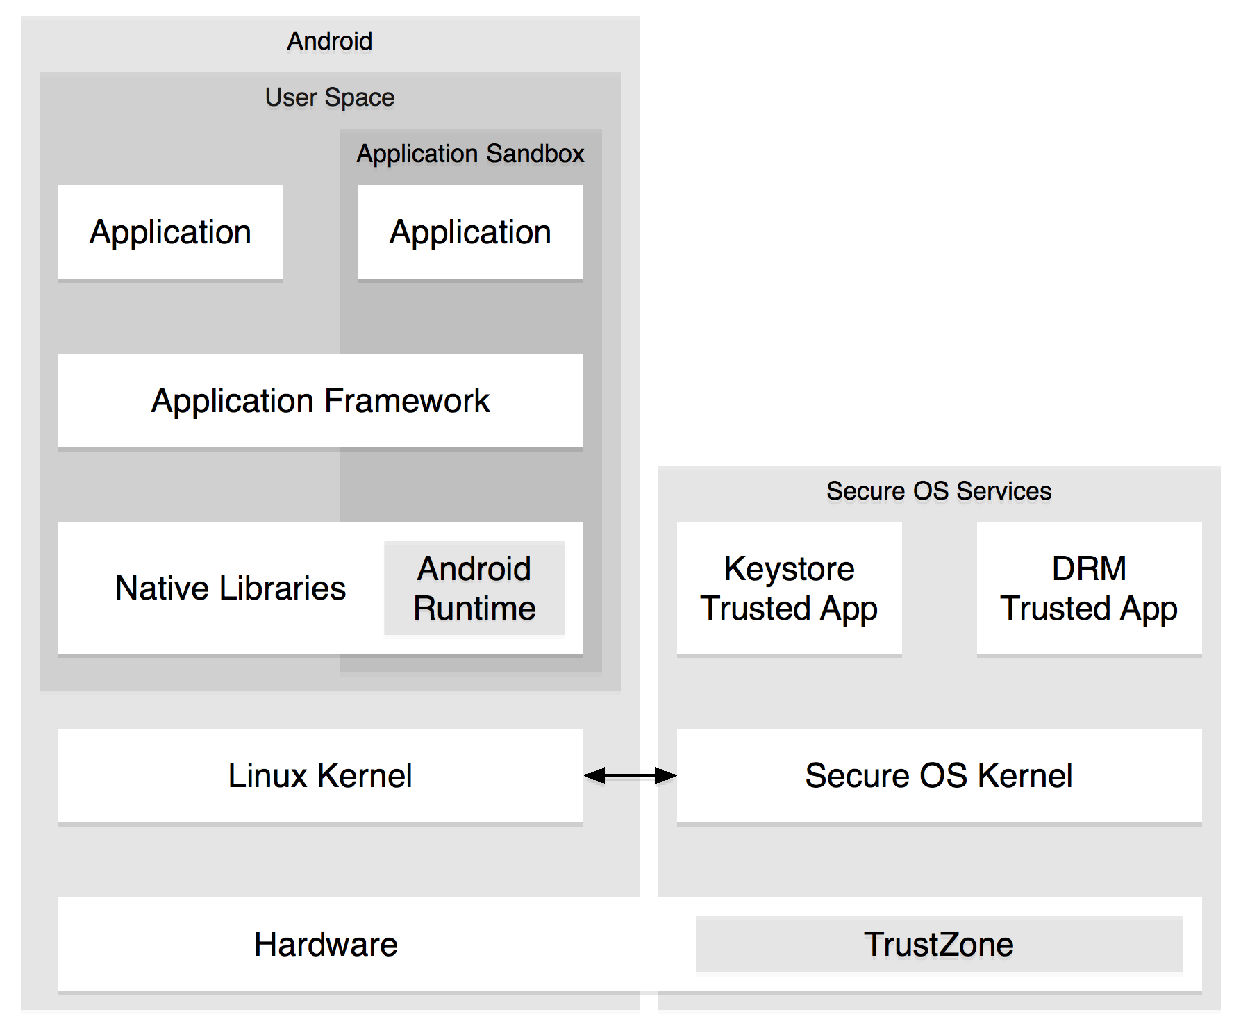
\includegraphics[width=1.0\linewidth]{chapters/02-mobile-ecosystems/figures/android-stack.eps}
  \caption{System stack of a typical Android device.}
  \label{fig:android_stack}
\end{figure}

\section{App stores and mobile app deployment}

\section{Android security model}



\section{Android policies}

\end{document}

%%% Local Variables:
%%% mode: latex
%%% TeX-master: "../../thesis"
%%% End:
